\documentclass[onecolumn]{IEEEtran}
\usepackage{amsmath}
\usepackage{amsfonts}
\usepackage{graphicx}
\usepackage{cite}
\usepackage{multirow}
\title{\textbf{PertNAS: Architectural Perturbations for Memory-Efficient Neural Architecture Search}}
\author{Keshav Mishra\\Indian Institute of Technology Bhilai\\Computer Science and Engineering\\12341140}
\date{}

\renewcommand{\abstractname}{}

\begin{document}

\maketitle

\begin{abstract}
	\textbf{\textit{Abstract}—Differentiable Neural Architecture Search (NAS) relies on aggressive weight-sharing to reduce its search cost. This leads to GPUmemory bottlenecks that hamper the algorithm’s scalability. To resolve these bottlenecks, we propose a perturbations-based evolutionary approach that significantly reduces the memory cost while largely maintaining the efficiency benefits of weight-sharing. Our approach makes minute changes to compact neural architectures and measures their impact on performance. In this way, it extracts high-quality motifs from the search space. We utilize these perturbations to perform NAS in compact models evolving over time to traverse the search space. Our method disentangles GPU-memory consumption from search space size, offering exceptional scalability to large search spaces. Results show competitive accuracy on multiple benchmarks, including CIFAR10, ImageNet2012, and NASBench-301. Specifically, our approach improves accuracy on	ImageNet and NASBench-301 by 0.3\% and 0.87\%, respectively. Furthermore, the memory consumption of search is reduced by roughly 80\% against state-of-the-art weight-shared differentiable NAS works while achieving a search time of only 6 GPU hours.}
\end{abstract}

\section{INTRODUCTION}
Neural Architecture Search (NAS) is paving the way for efficient and automated architecture designs that offer better accuracy/FLOPs tradeoffs compared to handcrafted models \cite{Howard2019}. Complex convolutional models consist of a number of control knobs – including architecture depth, operation choices, kernel sizes, and topologies – that govern their accuracy and computational/memory complexity. Tuning these control knobs by hand is a tedious process. NAS aims to automate this tuning process to achieve parameter-efficient models. However, the applicability of many NAS methods is limited by computation resources for two major reasons: 1) Model evaluation is costly \cite{Howard2019}-\cite{Tan2019}. Training all individual models in the search space is prohibitively time-consuming and resource-demanding. 2) Search spaces are limited by hardware resources. To reduce the exorbitant computational cost of NAS methods, experts often have to severely restrict the search space \cite{Zoph2017, Liu2018}, leading to serious inductive biases and sub-optimal solutions. These two reasons make NAS research fairly expensive and seriously limit the scalability of existing solutions.

Some NAS methods perform an exhaustive evaluation using search schemes like reinforcement learning (RL). They first train a large number of models sampled from the search space. Then the performance and architectures of these models are used to train a surrogate RL controller; usually an RNN, to further sample better architectures over time. Given the insurmountable number of model evaluations required to train the RL controller, RL-based methods require a huge amount of computation resources \cite{Zoph2017}. Take the MobileNetV3 \cite{Howard2019} as an example. Although these models remain unbeatable in terms of their parameter efficiency (accuracy/FLOPs), their RL-based searching process requires thousands of GPUs/TPUs over several days to weeks to be searched. Hence, these methods cannot be replicated within reasonable cost when applied to new datasets or tasks.

To mitigate such high demand on computation resources, differentiable architecture search approaches \cite{Liu2018}–\cite{Zela2019} adopt aggressive weightsharing \cite{Pham2018} between models in the search space. It allows evaluation of the search space components in a single-shot fashion, offering search costs as low as only a few GPU hours. However, the search space scalability of these methods is seriously limited due to the single-shot evaluation, which requires training models with sizes proportional to the search space size. It leads to prohibitive GPU memory consumption, which becomes one major bottleneck in the hardware constraints \cite{Cai2018, Xu2019}. To ensure a good result from a limited search space, experts carefully design these search spaces using knowledge obtained from high-quality manual neural architecture designs \cite{Zela2020, Siems2020}. This inevitably adds significant inductive bias to the search process \cite{Zoph2017}. Furthermore, the effectiveness of the differentiable search methods has been questioned repeatedly \cite{Zela2019, Li2020}, whereby random search has outperformed differentiable search approaches \cite{Li2020}. Their weight-sharing technique \cite{Pham2018} has been shown to suffer from a rank miscorrelation problem whereby weight-shared models are known to serve as poor surrogates for full model training \cite{Zela2020, Zhang2020, Pourchot2020}.

In this work, we propose an evolutionary search scheme that utilizes architectural ‘perturbations’ as an evaluation metric to identify high-quality components of the search space. This search scheme evaluates and evolves compact models over time to explore the search space. It circumvents the severe memory limit faced by one-shot NAS methods. During searching, we apply small changes to neural architectures, called perturbations, and measure their impact on the model performance. This helps to identify high-quality motifs from search spaces. We demonstrate that perturbations offer more efficient, scalable, and verifiable operation strength evaluation over black-box differentiable approaches.

The contributions of this work are as follows:
\begin{enumerate}
	\item We explore architectural perturbations as an operation strength evaluation metric for NAS. We are the first to explore perturbations as the basis to perform NAS without using overparametrized models, addressing their memory bottlenecks.
	\item We propose a perturbations-based evolutionary approach that relies only partially on weight-sharing and serves as a fast, accurate, and scalable search method. Our method achieves a search cost of only 6 GPU-hours with peak memory consumption of only 20\% that of differentiable approaches. Furthermore, experimentation on ImageNet and NASBench-301 shows an improvement of 0.3\% and 0.87\% in accuracy, respectively, against state-of-the-art in differentiable NAS.
	\item The memory consumption of PertNAS does not depend on search space size. It is similar to training a single compact model sampled from the search space. In comparison, existing differentiable search works \cite{Liu2018, Wang2021} all require GPU memory that scales linearly with search space size. Disentangling the size from memory-cost paves the way for scaling up the search space, which proves to produce better models \cite{Howard2019}.
\end{enumerate}

\section{PRELIMINARIES}
\subsection{Background}
\textbf{Search Spaces.} Search spaces represent the control knobs that require tuning. Most one-shot NAS approaches, such as DARTS \cite{Liu2018} and its variants \cite{Wang2021, Zela2019} employ a repeating cell-based search space. This alleviates the search cost to that of searching for cells instead of an entire neural network. A cell is represented by a directed acyclic graph (DAG) where nodes represent feature maps while edges represent operations. The DARTS cells utilize two input nodes, four intermediate nodes, and one output node. The two input nodes are the outputs of the two previous cells, while each successive intermediate node takes its input from all previous nodes. The feature map representing an intermediate node is calculated by applying the operations on each of its incoming edges to their respective input nodes. The output of the k-th cell, \( c_k \), is obtained by concatenating the feature maps represented by the intermediate nodes along the channel dimension. Figure~\ref{fig:architecture_search} (a) top shows a cell with one input, one output, and two intermediate nodes – in green, yellow, and blue colors, respectively. DARTS and its variants employ two types of cells: normal cells with stride one operations and reduction cells with stride two operations to reduce the spatial resolution. Cells resulting from the search phase are replicated as part of a larger model for evaluation. For example, an evaluation model for CIFAR10 utilizes 18 normal and two reduction cells. Since reduction cells serve only to reduce spatial resolution, we utilize the same architecture for normal and reduction cells but with stride two operations in reduction cells. \\
The DARTS search space consists of 8 operations which include a skip connect, two pooling, two separable, and two dilated convolutions. This work considers the baseline DARTS search space \( O_D \) along with two compact variants listed in Table~\ref{tab:search_spaces}. The variants allow exhaustive evaluation and ablation studies to be performed, given that the baseline DARTS search space is too large to be evaluated exhaustively with \(\sim 10^{25}\) models.

\begin{figure}[ht]
	\centering
	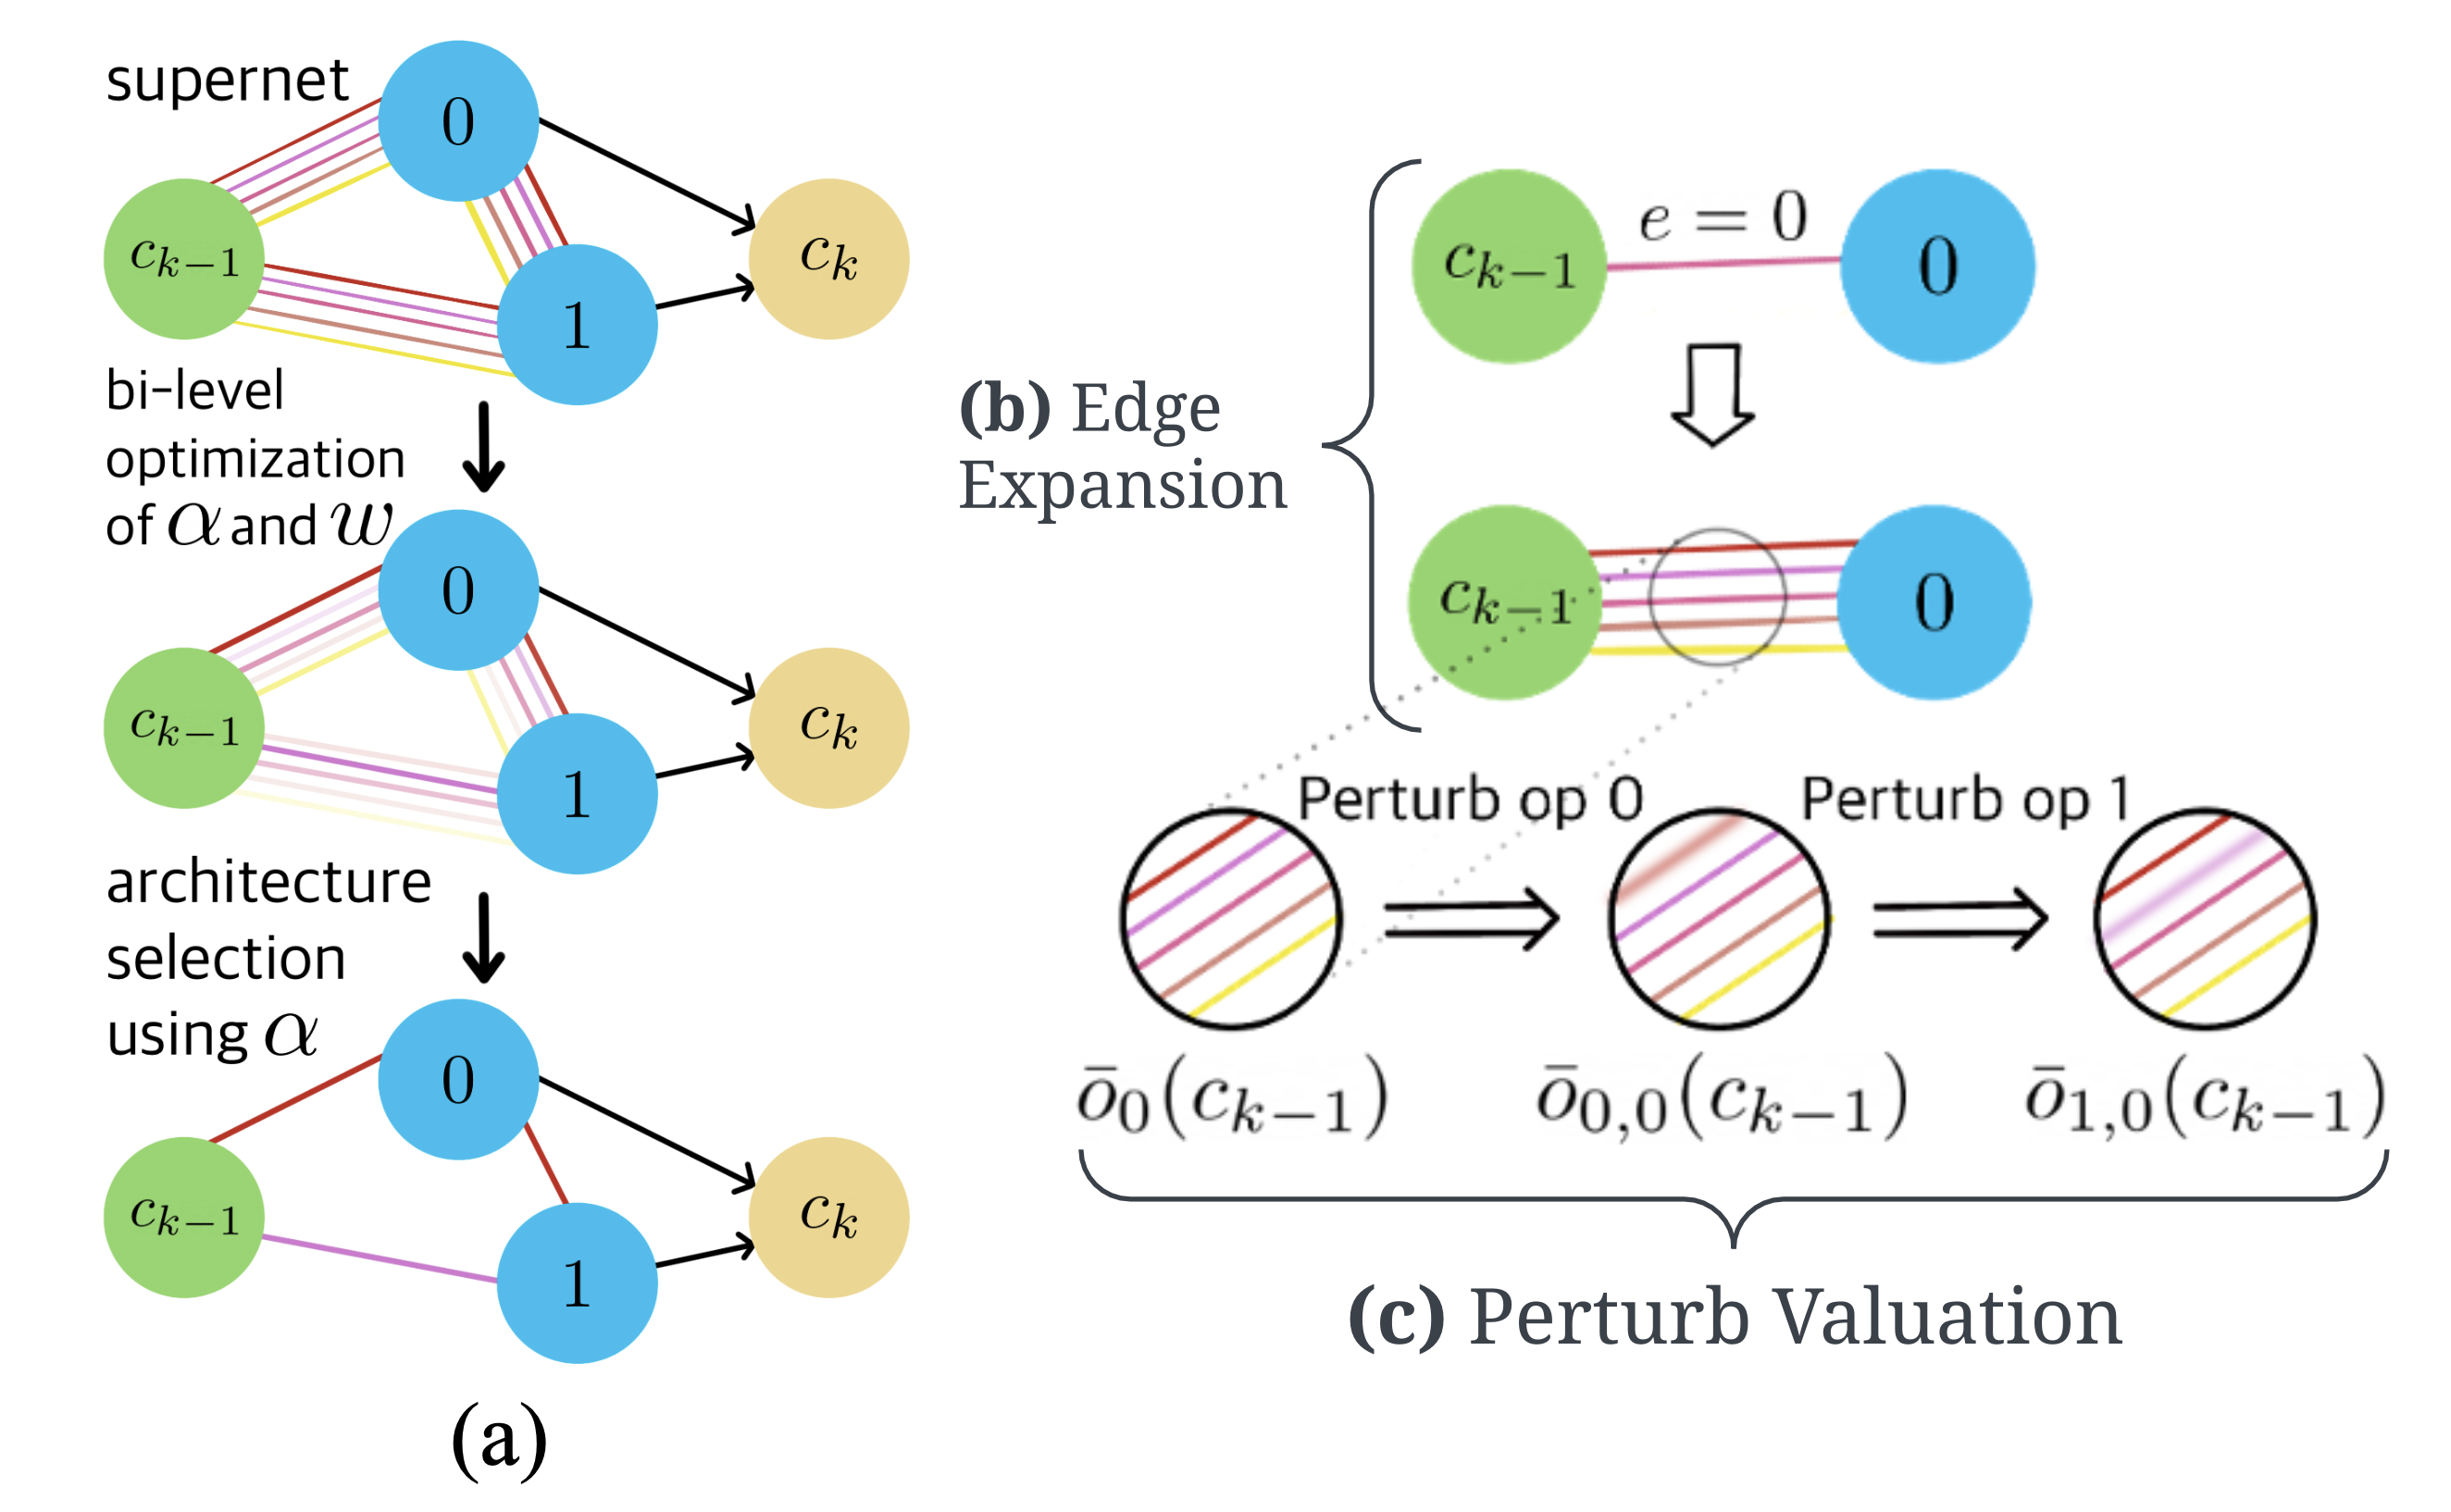
\includegraphics[width=0.5\textwidth]{Figure-1.png}
    \caption{(a) Differentiable architecture search \cite{Liu2018} performs a bi-level optimization on a weight-shared supernet to jointly optimize architecture \( \alpha \) and weights \( w \). (b) Expansion of an edge involves placing all operations in \( O \) on that edge. (c) Perturb valuation of an operation strength is performed by masking that operation when measuring the output of mixed operation \( \bar{o}_{m,e} \) (masked operations represented by blurred lines in inset).}
	\label{fig:architecture_search}
\end{figure}

\textbf{Search Progression.} The goal of the search is to find high-quality operations and connections within the cells. Specifically, DARTS-like works aim to find top-2 incoming edges per intermediate node (topology search) and the best operation per edge (operation search). We follow a 3-step approach in our search progression: 1) Coarse- grained operation search for eliminating low-quality operations from the search space in an approximate fashion with little search cost, 2) Fine- grained operation search for selecting the best operation on each edge (discretization of each edge) with high accuracy, and 3) Topology search for finding top-2 incoming edges for each intermediate node (discretization of each node) as per the goal of DARTS \cite{Liu2018}. Dividing the search into these three steps reduces search cost significantly by performing the search at different scales; approximate and low-cost in the early stages, accurate and high-cost in later stages.

\subsection{Related Works}
\textbf{Differentiable NAS.} In recent years, differentiable one-shot approaches have gained traction due to their ability to jointly optimize a weight-shared supernet architecture and its network weights for efficient search \cite{Liu2018, Xu2019, Xie2018}. DARTS \cite{Liu2018} represents the search space by relaxing the categorical choice of a candidate

\begin{table}[ht]
	\centering
	\caption{Search Spaces Considered in This Work.}
	\label{tab:search_spaces}
	\begin{tabular}{ccccc}
		\hline
		Search Space & Candidate Operations, $\mathcal{O}$ & $\left|\mathcal{O}\right|$ & $\left|\mathcal{E}\right|$ & Topology\\
		\hline
		$\mathcal{O}_D$ & DARTS \cite{Liu2018} & 8 & 14 & Flexible\\
		$\mathcal{O}_1$ & \{skip connect, max pool 3x3, sep conv 3x3, sep conv 5x5\} & 4 & 8 & Shallow (d=1)\\ 
		$\mathcal{O}_2$ & Best ops for each edge in $\mathcal{O}_1$ & 1 & 14 & Flexible\\ \hline
		\end{tabular}
	\end{table}
 
 operation to a softmax over all possible operations in the form of an overparametrized ‘supernet’ (Figure~\ref{fig:architecture_search} (a), Top, Different colors on edges represent different operations in the candidate operation set). A supernet is a DAG representation of the search space that consists of all possible operations and topology connections that can be constructed from it. Each edge of the DAG consists of all candidate operations, represented by \( O \). The output of an edge, called a mixed operation, is the weighted sum of operations on that edge applied to the input. The weights associated with the candidate operations are parametrized by a vector \( \alpha \) which represents the relative strength of their corresponding operations. The output of a mixed operation on edge \( e \in E \), where \( E \) is the list of all edges, is given as
\begin{equation}
\overline{o}_e(x) = \frac{\sum_{o \in O} \exp(\alpha_{e,o}) o(x)}{\sum_{o' \in O} \exp(\alpha_{e,o'})}
\label{eq:exp}
\end{equation}
Where \( O \) represents the candidate operations in the search space and \( o(x) \) represents an operation \( o \) to be applied to the input feature map \( x \). A bi-level optimization is utilized to jointly learn both architecture \( \alpha \) as well as the network weights \( w \) (Figure~\ref{fig:architecture_search} (a), Center, Opacity represents operation value/strength, \( \alpha \)):
\begin{equation}
\min_{\alpha} L_{\text{val}}(w^*(\alpha), \alpha) \quad \text{s.t.} \quad w^*(\alpha) = \arg\min_{w} L_{\text{train}}(w, \alpha)
\label{eq:arg}
\end{equation}
The final architecture is obtained by choosing the operations corresponding to the highest \( \alpha \) (Figure~\ref{fig:architecture_search} (a), Bottom, Only branches with highest opacity on each edge remain).

\textbf{Memory-Efficient NAS.} DARTS \cite{Liu2018} is known to suffer from memory bottleneck issues \cite{Cai2018, Xu2019}. The DARTS supernet consumes roughly \(|O| \times\) the GPU memory of a single model in the search space. Hence, DARTS-like approaches impose search space size limits due to the memory limits of the hardware. ProxylessNAS \cite{Cai2018} proposed a solution in the form of binarized architecture paths. During the training of the supernet, only one of the \(|O|\) paths is activated using stochastically sampled binary gates, leading to a memory cost roughly the same as that of training a single compact model. However, the search cost of over 8 GPU-days and model sizes \(\sim 70\%\) greater than DARTS, combined with only a modest improvement in accuracy, makes the approach less appealing. PC-DARTS \cite{Xu2019} proposed another solution to the memory bottlenecks by sampling partial channel connections of the supernet during the search. This approach relies on performing the operation search using only a subset of feature map channels. However, the reproduced results of PC-DARTS \cite{Xu2019} show unremarkable improvements over existing works in accuracy.

\textbf{Perturbation methods.} The success of deep learning comes from exploiting infinitesimal perturbations at an enormous scale. Stochastic gradient descent applies minuscule perturbations to the weights of a model so that, over time, the model weights satisfy the objective function better. Hence, it is natural to ask whether perturbations can also be exploited at an architectural level. DARTS+PT \cite{Wang2021} showed that perturbing DARTS-optimized supernets can help evaluate and remove weak operations and connections from the search space. Our work is closely related to DARTS+PT but explores architectural perturbations as the basis to perform NAS without using gradient-based optimization utilized by DARTS-like works.

\begin{figure}[ht]
	\centering
	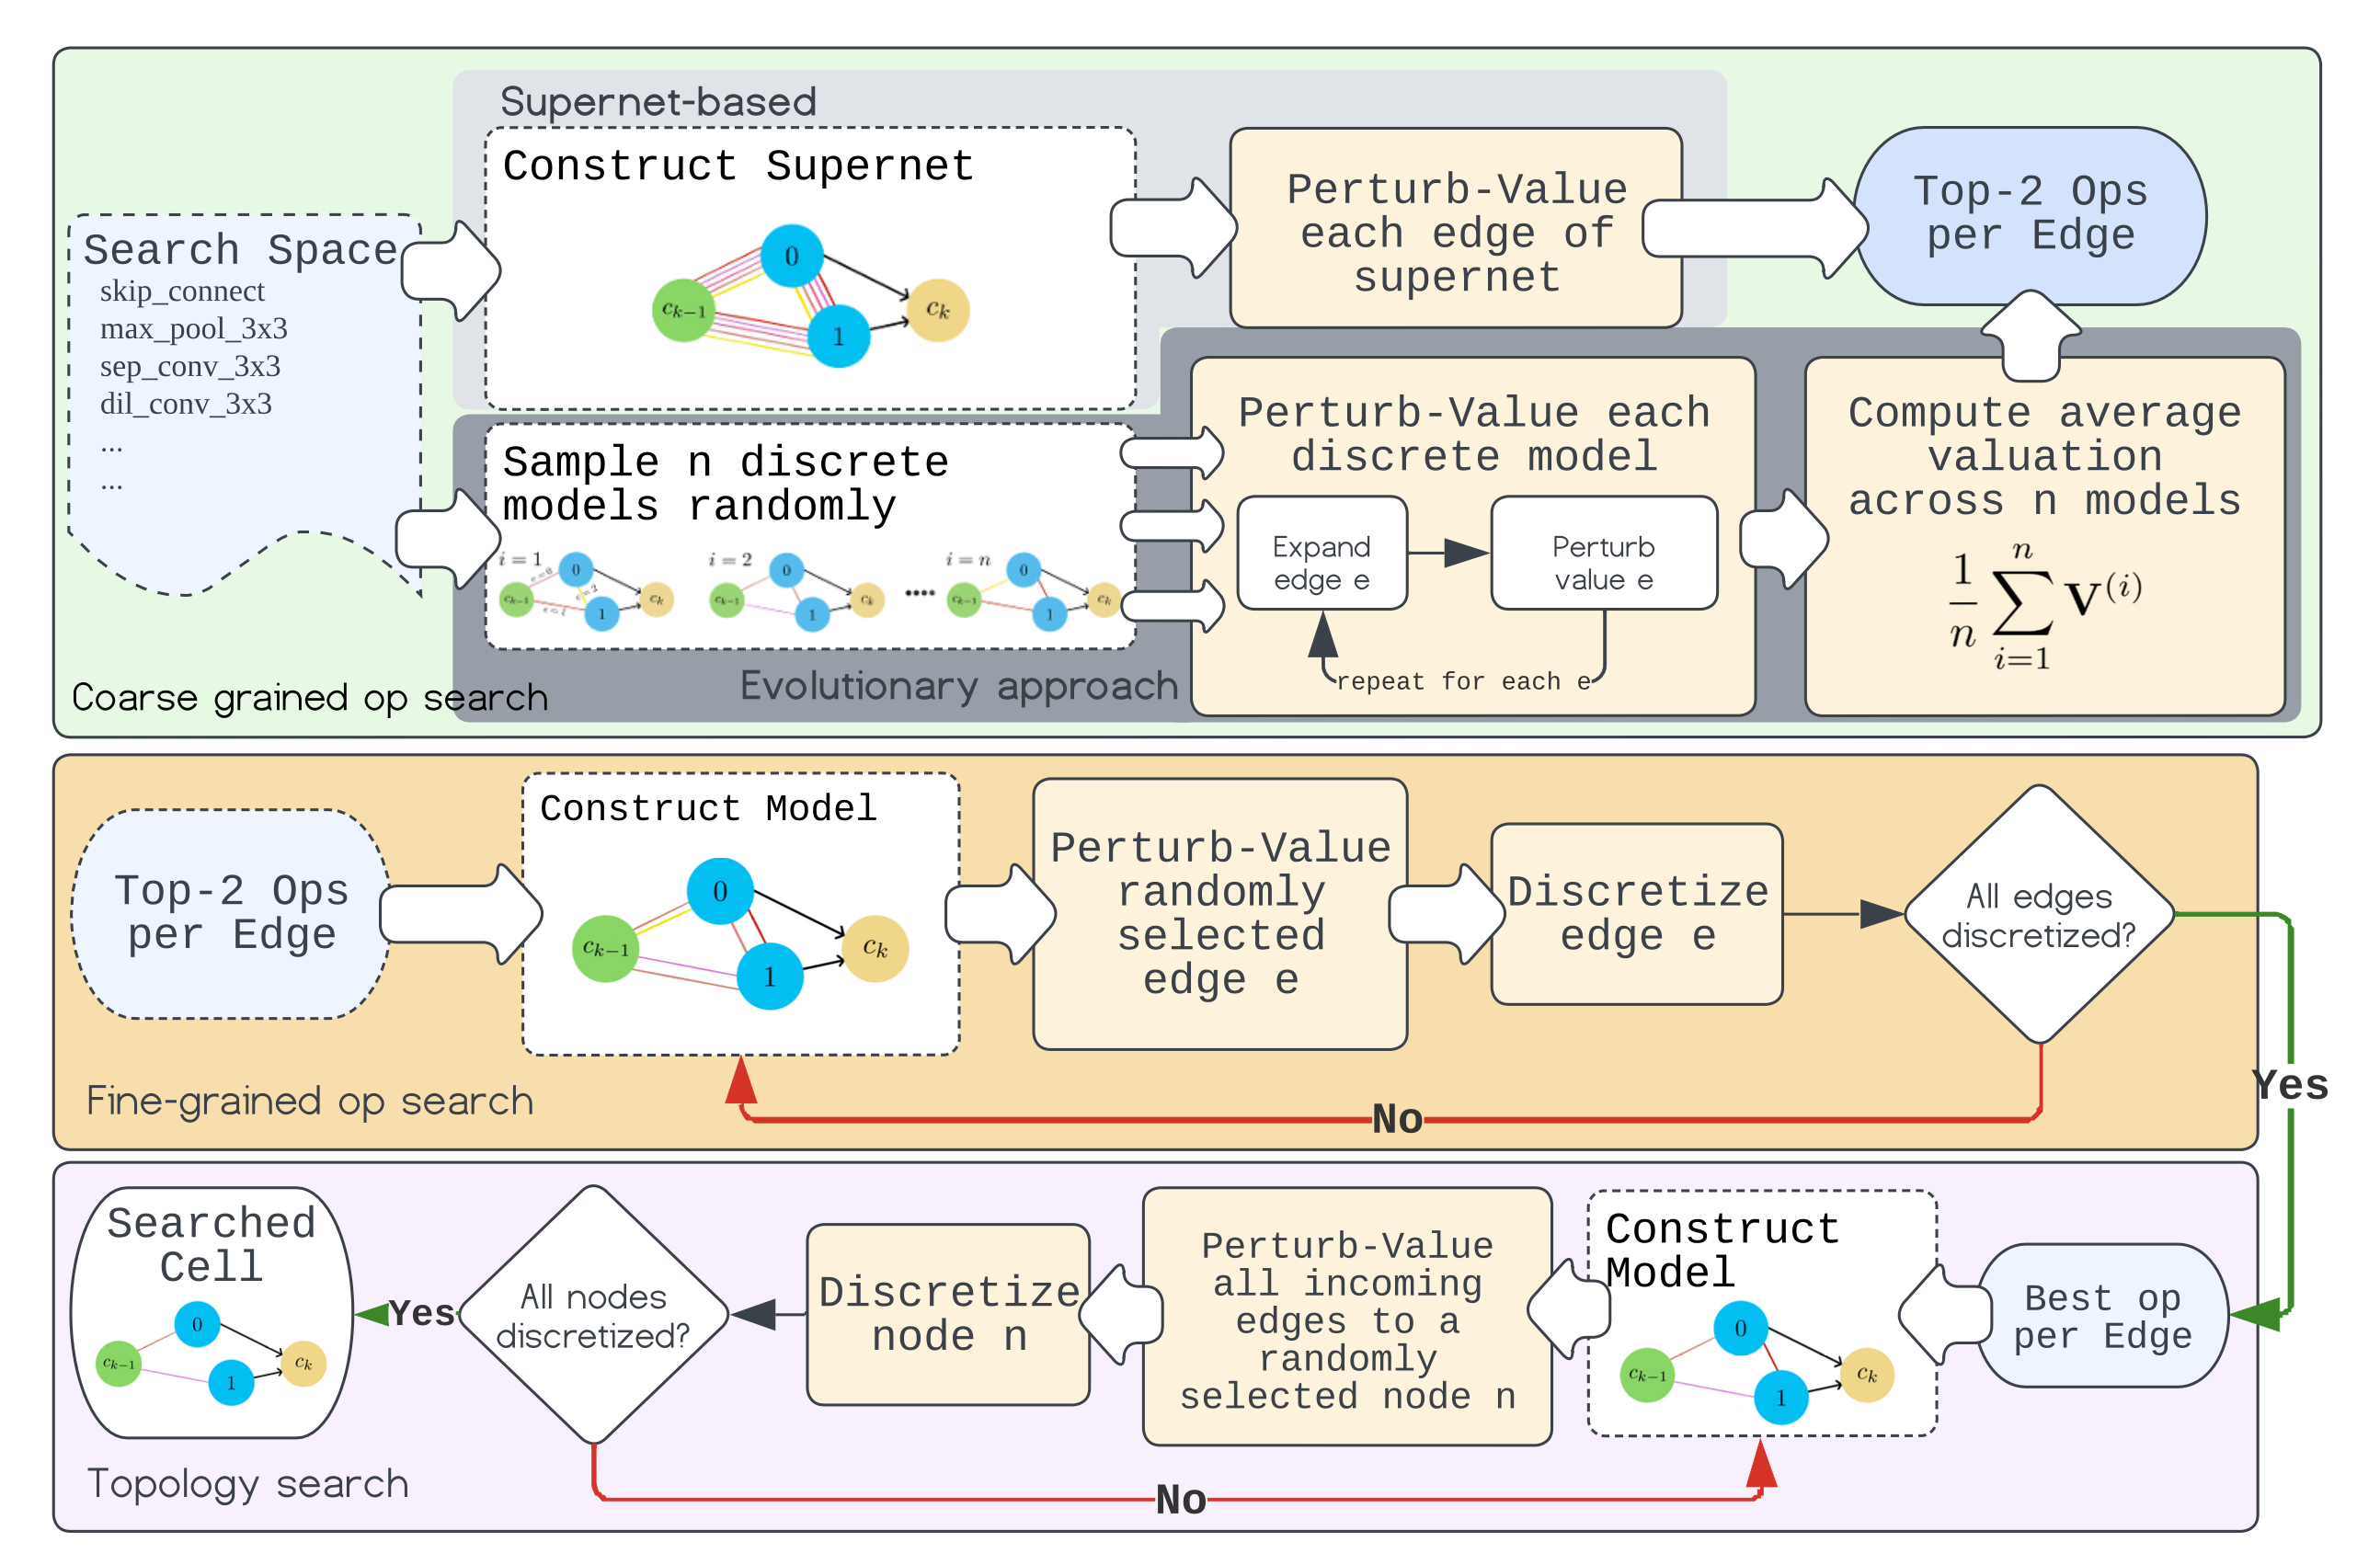
\includegraphics[width=0.5\textwidth]{Figure-2.png}
	\caption{Flowchart of our perturbations-based search. Supernet-based search relies on training a large supernet (light gray) while the evolutionary approach relies on performing operation valuation from within \( n \) discrete models (dark gray) using expansion followed by perturb valuation.}
	\label{fig:flowchart_search}
\end{figure}

\section{SEARCH METHOD}

\subsection{Perturbations-based Evaluation}
\textbf{Approach.} We explore a perturbations-based approach to identify high-quality components of the search space. Perturbations to an operation \( o \) on edge \( e \) refer to the removal of the operation from that edge. This is implemented by masking the corresponding operation as shown in Figure~\ref{fig:architecture_search} (c). The output of the masked mixed operation \( \bar{o}_{m,e} \), which denotes operation \( m \) masked on edge \( e \), is given by:

\begin{equation}
	\bar{o}_{m,e}(x) = \sum_{o \in O} 1_{o \neq m} \cdot o(x)
	\label{eq:sum}
\end{equation}

Where the mask vector \( 1 \) is the indicator function. Comparing the output of the mixed operation of our approach in Eq.~\ref{eq:sum} with that of differentiable approaches in Eq.~\ref{eq:exp}, we note that we do not utilize \( \alpha \) to represent operation strength. Instead, in our approach, the value/strength of the operation \( o \) on edge \( e \), denoted by \( \Delta V_{o,e} \), is defined as the change in accuracy resulting from the perturbation of \( o \) on edge \( e \):

\begin{equation}
	\Delta V_{o,e} = V_{o,e} - V^*
	\label{eq:validation}
\end{equation}

Where \( V^* \) is the validation accuracy of the unperturbed model, and \( V_{o,e} \) is the accuracy when a perturbation is applied to \( o \) on \( e \). The meaning of \( \Delta V_{o,e} \) is reasonably intuitive to interpret: it is the degradation in accuracy of the model when operation \( o \) is removed from edge \( e \), signifying the contribution of \( \{o,e\} \) towards the accuracy of the model.

\textbf{Approximation of Accuracy of Perturbed Models.} For measuring operation strength, or valuation (Eq.~\ref{eq:validation}), \( V^* \) can be obtained trivially by training the unperturbed model to convergence. However, since perturbed and unperturbed models have different architectures, obtaining \( V_{o,e} \) is non-trivial since it needs to be obtained from the perturbed model with \( \{o,e\} \) pair removed/masked. Let \( s^*_{\theta}(x) \) and \( s_{(o,e),\theta'}(x) \) be the unperturbed model with parameters \( \theta \) and perturbed model with parameters \( \theta' \), respectively. It follows that \( \theta' \neq \theta \) given \( s_{(o,e)}(x) \neq s^*(x) \). Training \( s_{(o,e),\theta'}(x) \) from scratch to convergence is computationally impractical, given that this needs to be performed for each \( o,e \) pair. For a sufficiently small perturbation to the model such that the base and perturbed model architectures are fairly similar (i.e., \( s^*(x) \sim s_{(o,e)}(x) \)), \( \theta' \) can be approximated from \( \theta \) by sharing the weights of the base model with those of the perturbed model and finetuning the perturbed model. This allows \( V_{o,e} \) to be estimated from \( s_{(o,e),\theta'}(x) \) using \( \theta' \sim \theta \) as the parameter initialization for the perturbed model in a computationally tractable manner.


\subsection{Search Flow using Supernets}
Figure~\ref{fig:flowchart_search} shows a flowchart of our approach detailing the three-stage search progression highlighted in Sec. II-A. Please note that cells depicted in Fig.~\ref{fig:flowchart_search} are simplified variants of the real cells used in experiments for ease of visualization. The actual cells utilize two input and four intermediate nodes as per the cell template utilized by DARTS \cite{Liu2018} and its variants \cite{Liu2018, Xu2019, Xie2018} for fair comparison. Operation search is divided into two stages of different granularities; coarse- and fine-grained search. Coarse-grained search eliminates weak operations in a low-cost fashion. In contrast, fine-grained search caters to the operation search goal by discretizing edges of the DAG in succession and with high confidence. 

In coarse-grained operation search, we utilize perturbations to obtain valuations of all operations in the search space. We utilize two approaches to perform this valuation. The first approach, supernet-based search, shown in light gray in Fig.~\ref{fig:flowchart_search} (top), utilizes perturbations on a supernet to obtain the valuation of all operations on each edge of the DAG. Specifically, we construct a supernet cell by placing all search space operations \( O \) onto each edge of the DAG. Eight cells are connected sequentially to form the search network, whereby cell \( k \) takes its input from the two previous cells, \( k-1 \) and \( k-2 \). 

After training the search network \( s^*_{\theta}(x) \) to convergence and obtaining \( V^* \), we perform the valuation of search space using the perturbations-based approach. To measure the strength of operation \( o \) on an edge \( e \), we mask \( o \) on \( e \) to construct \( s_{(o,e),\theta'}(x) \). We then initialize \( \theta' \) with \( \theta \), i.e., \( s_{(o,e)}^{\theta'}(x) = s_{\theta}(x) \), and finetune this perturbed model so \( s_{(o,e)}(x) \) reaches convergence. The validation accuracy of this perturbed model \( V_{o,e} \) is used to calculate \( \Delta V_{o,e} \). The process of evaluating \( o \) and \( e \) is repeated for all \( o \in O \) and \( e \in E \) to obtain the valuation matrix \( V \in \mathbb{R}^{|E| \times |O|} \), which represents the strength of each operation on each edge. For the DARTS search space \( O_D \), this corresponds to \( |O| = 8 \) and \( |E| = 14 \). The valuation matrix \( V \) is utilized to select the top-2 operations for each edge, i.e., the operations that cause the most degradation of accuracy when perturbed.

Fine-grained operation search (Fig.~\ref{fig:flowchart_search} center) starts by training a model constructed by sequentially connecting eight cells containing only the top-2 operations per edge. We then select and perturb-value operations on a random edge \( e \). We discretize \( e \) by selecting the best operation for \( e \) using the valuation and construct and train the new model with \( e \) discretized. We repeat this process until all edges in \( E \) have been discretized. The generated model is sparse and consists only of the best operation for each edge. Topology search (Fig.~\ref{fig:flowchart_search} bottom) follows the same process as fine-grained operation search but discretizes nodes instead of edges. This entails selecting top-2 incoming edges for each of the intermediate nodes.

Existing works have highlighted the memory bottlenecks presented by supernets \cite{Cai2018, Xu2019}. Specifically, a supernet consumes roughly \( |O| \times \) the memory of a single model in the search space. This places restrictions on search space sizes owing to hardware limitations. In the following subsection, we demonstrate how GPU memory required for search can be disentangled from the search space size.

\subsection{Disentangling Mem Consumption from Search Space Size}
Supernets have enjoyed much of their success owing to weight-sharing; each sub-network can inherit its weights from the supernet, bypassing the need for exhaustively training each sub-network independently. However, numerous works have exposed the rank miscorrelation problem in weight sharing, whereby weight-shared discrete architectures serve as poor surrogates for 
\begin{figure}[ht]
	\centering
	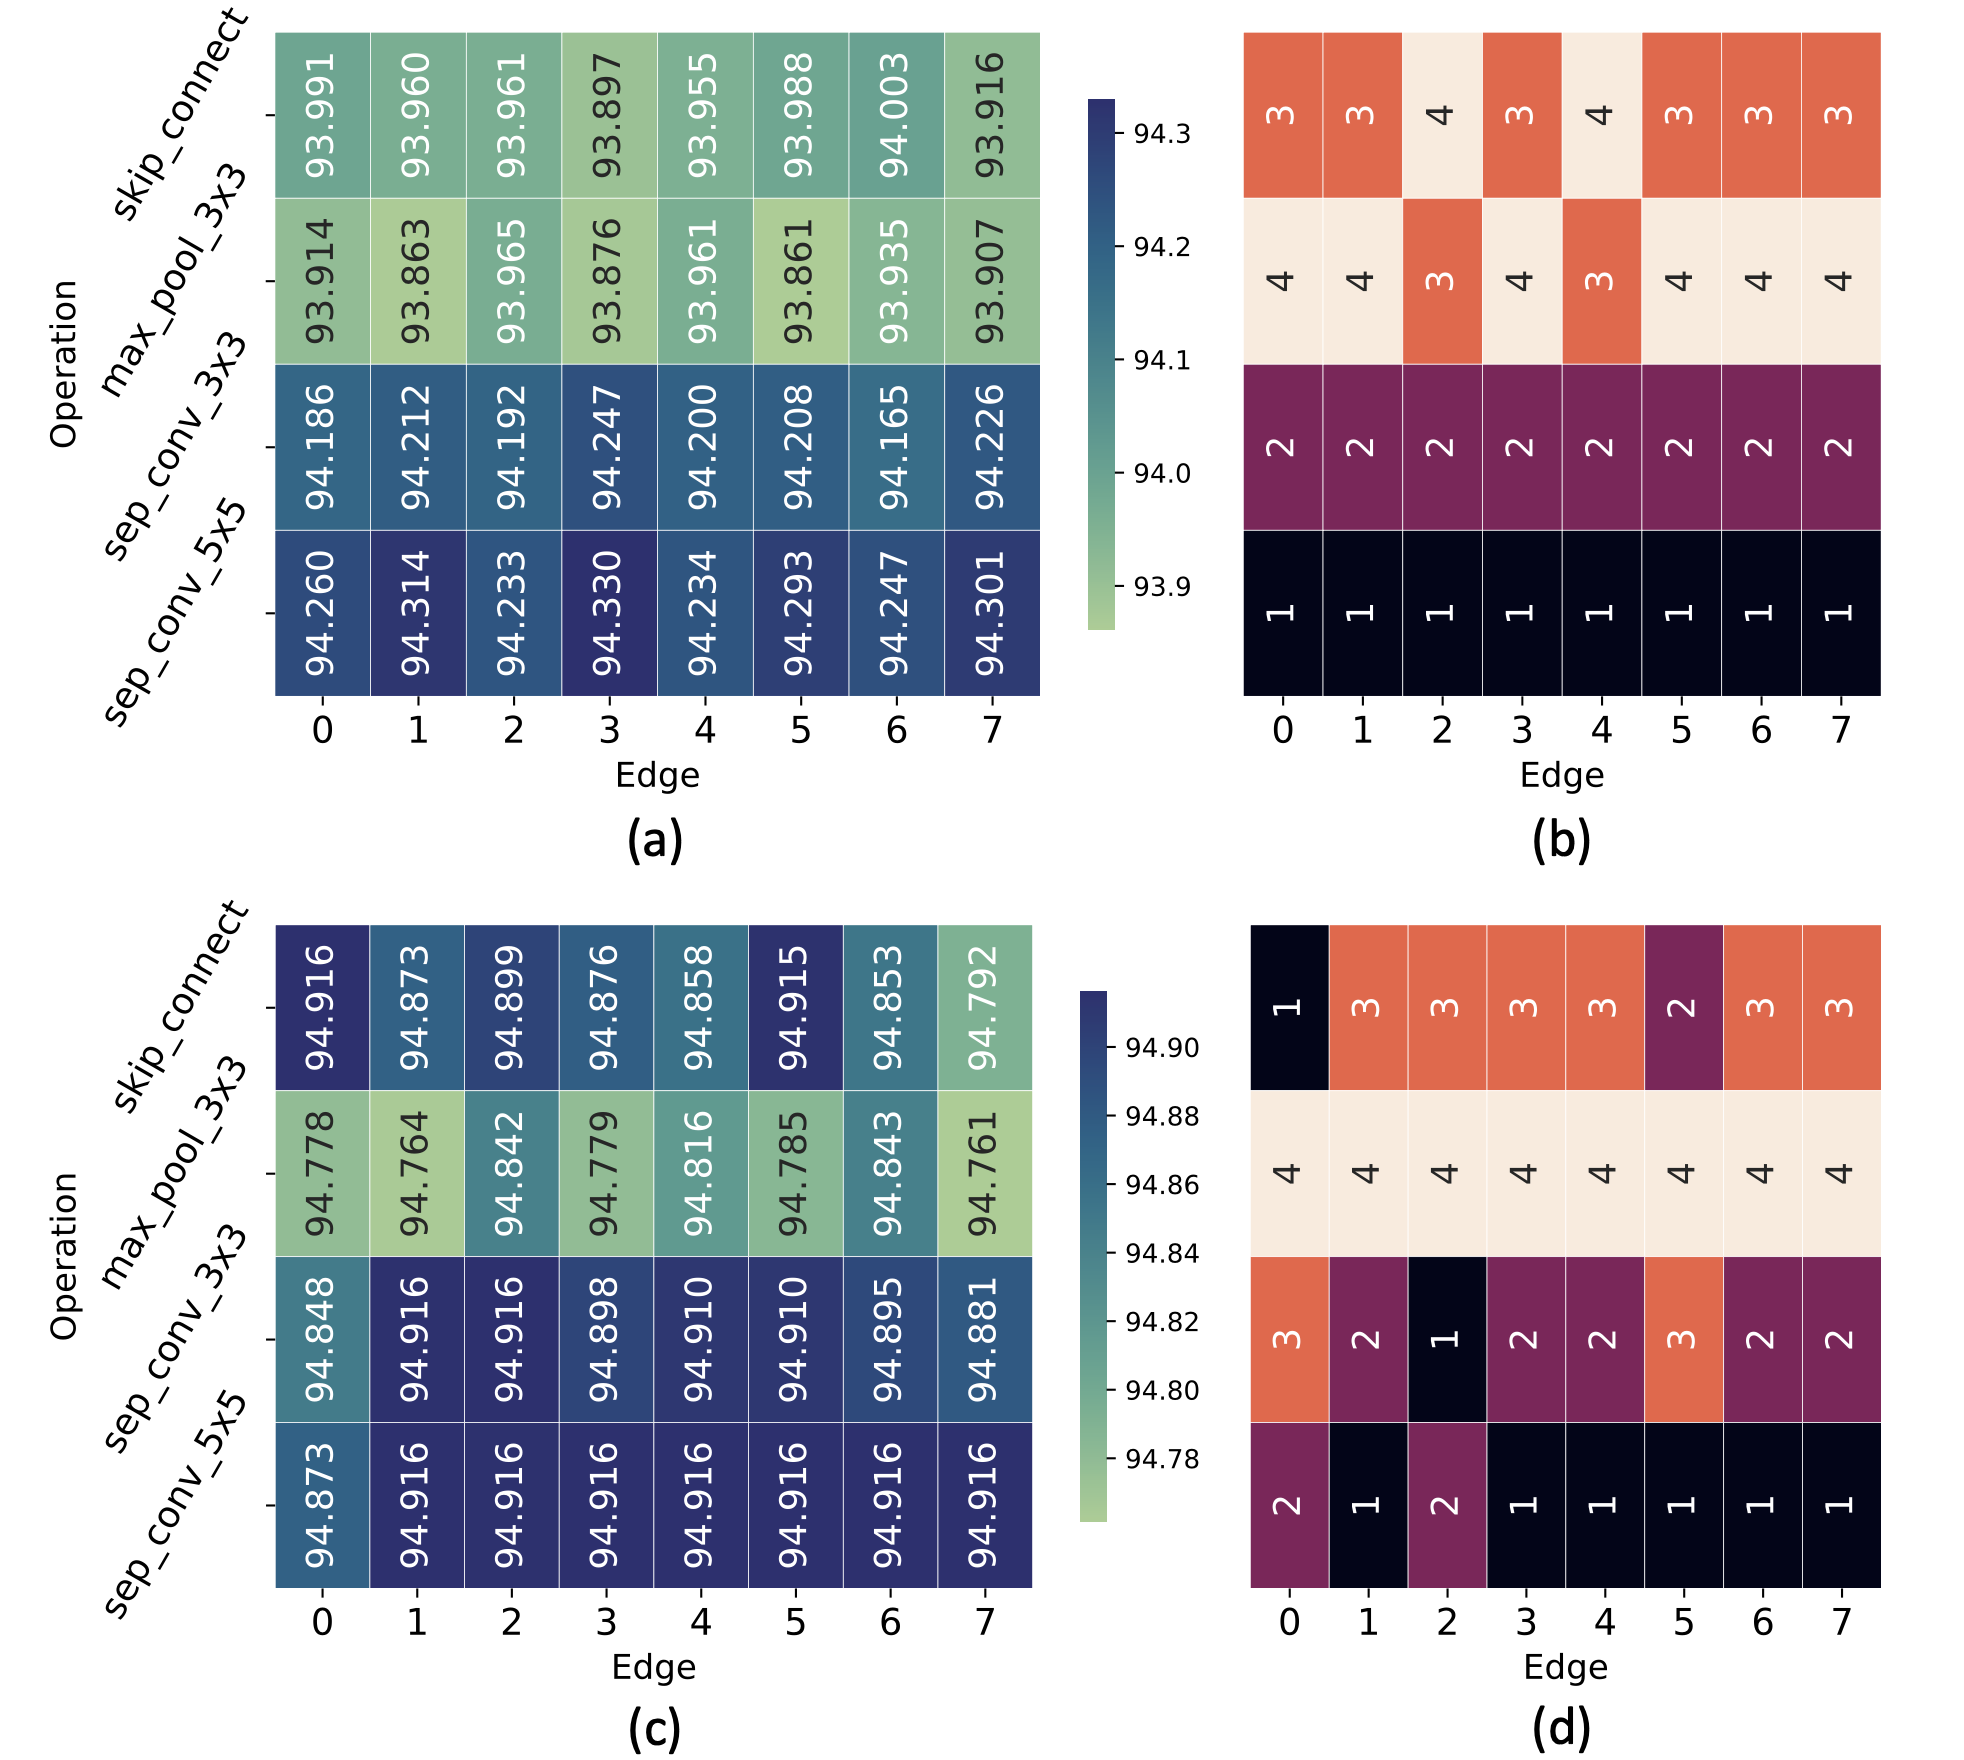
\includegraphics[width=0.45\textwidth]{Figure-3.png}
	\caption{Heatmaps of valuations and rankings obtained using (a)-(b) averaging architecture accuracies, and (c)-(d) obtaining accuracy of best model. They indicate that the rankings obtained by averaging model accuracies are fairly similar to rankings when best accuracy is selected for each operation choice.}
	\label{fig:heatmaps}
\end{figure}
full model training \cite{Zela2020, Zhang2020, Pourchot2020}. Furthermore, high memory consumption of supernets imposes restrictions on search space size \cite{Cai2018, Xu2019}. 

We show that the performance of operations is not necessarily tied to the edge they are located in relative to the other edges. This would mean that operations on each edge can be valued independently without sharing weights between operations on the remaining edges. 

 We obtain the accuracies of all \( |O|^{|E|} = 4^8 \sim 65k \) models in the \( O_1 \) search space on NASBench-301 \cite{Siems2020}. We compute the average accuracy of all possible discrete models (i.e., a model with one operation per edge) that can be constructed from making each operation selection on each edge (e.g., if we discretize edge 0 to the skip connect operation, we can construct a total of \( 47 \sim 16.4k \) different architectures). Similarly, we also obtain the accuracies of the best discrete model that can be constructed by discretizing each operation on each edge. Fig.~\ref{fig:heatmaps} shows heatmaps and operation importance rankings of the average and best accuracies of the remaining discrete architectures in the search space when each operation is discretized on each edge. We make two observations from these rankings: (1) Average rankings of operations are fairly consistent across all edges, i.e., some operations are almost always better than others, and (2) Top operations based on average and best rankings are fairly similar, i.e., the fact that sep conv 5x5 and 3x3 are the best operations for almost all edges is consistent between the two rankings. Since averaging the performance of models gives a good indicator of operation importance, we conclude that operations on edges can be valued independently.

\subsection{From Supernets to Evolutionary Search}
Based on the idea that each edge can be valued in isolation while the remaining edges need not be overparametrized, we propose an evolutionary approach that does not rely on supernets. Figure~\ref{fig:flowchart_search} (dark gray) shows the coarse-grained operation search phase using this evolutionary technique. We randomly sample a population of \( n \) discrete models from the search space and train each model to convergence. A discrete model refers to a model with only one operation per edge. For each model, we then expand an edge, finetune the model with the expanded edge, and apply perturb-valuation on this edge according to the approach detailed in Sec. III-A. Expanding an edge refers to loading all candidate operations to that edge, as shown in Figure~\ref{fig:architecture_search} (b). After obtaining the valuation of operations on this edge, we discretize this edge according to the valuation, expand the
\begin{figure}[ht]
	\centering
	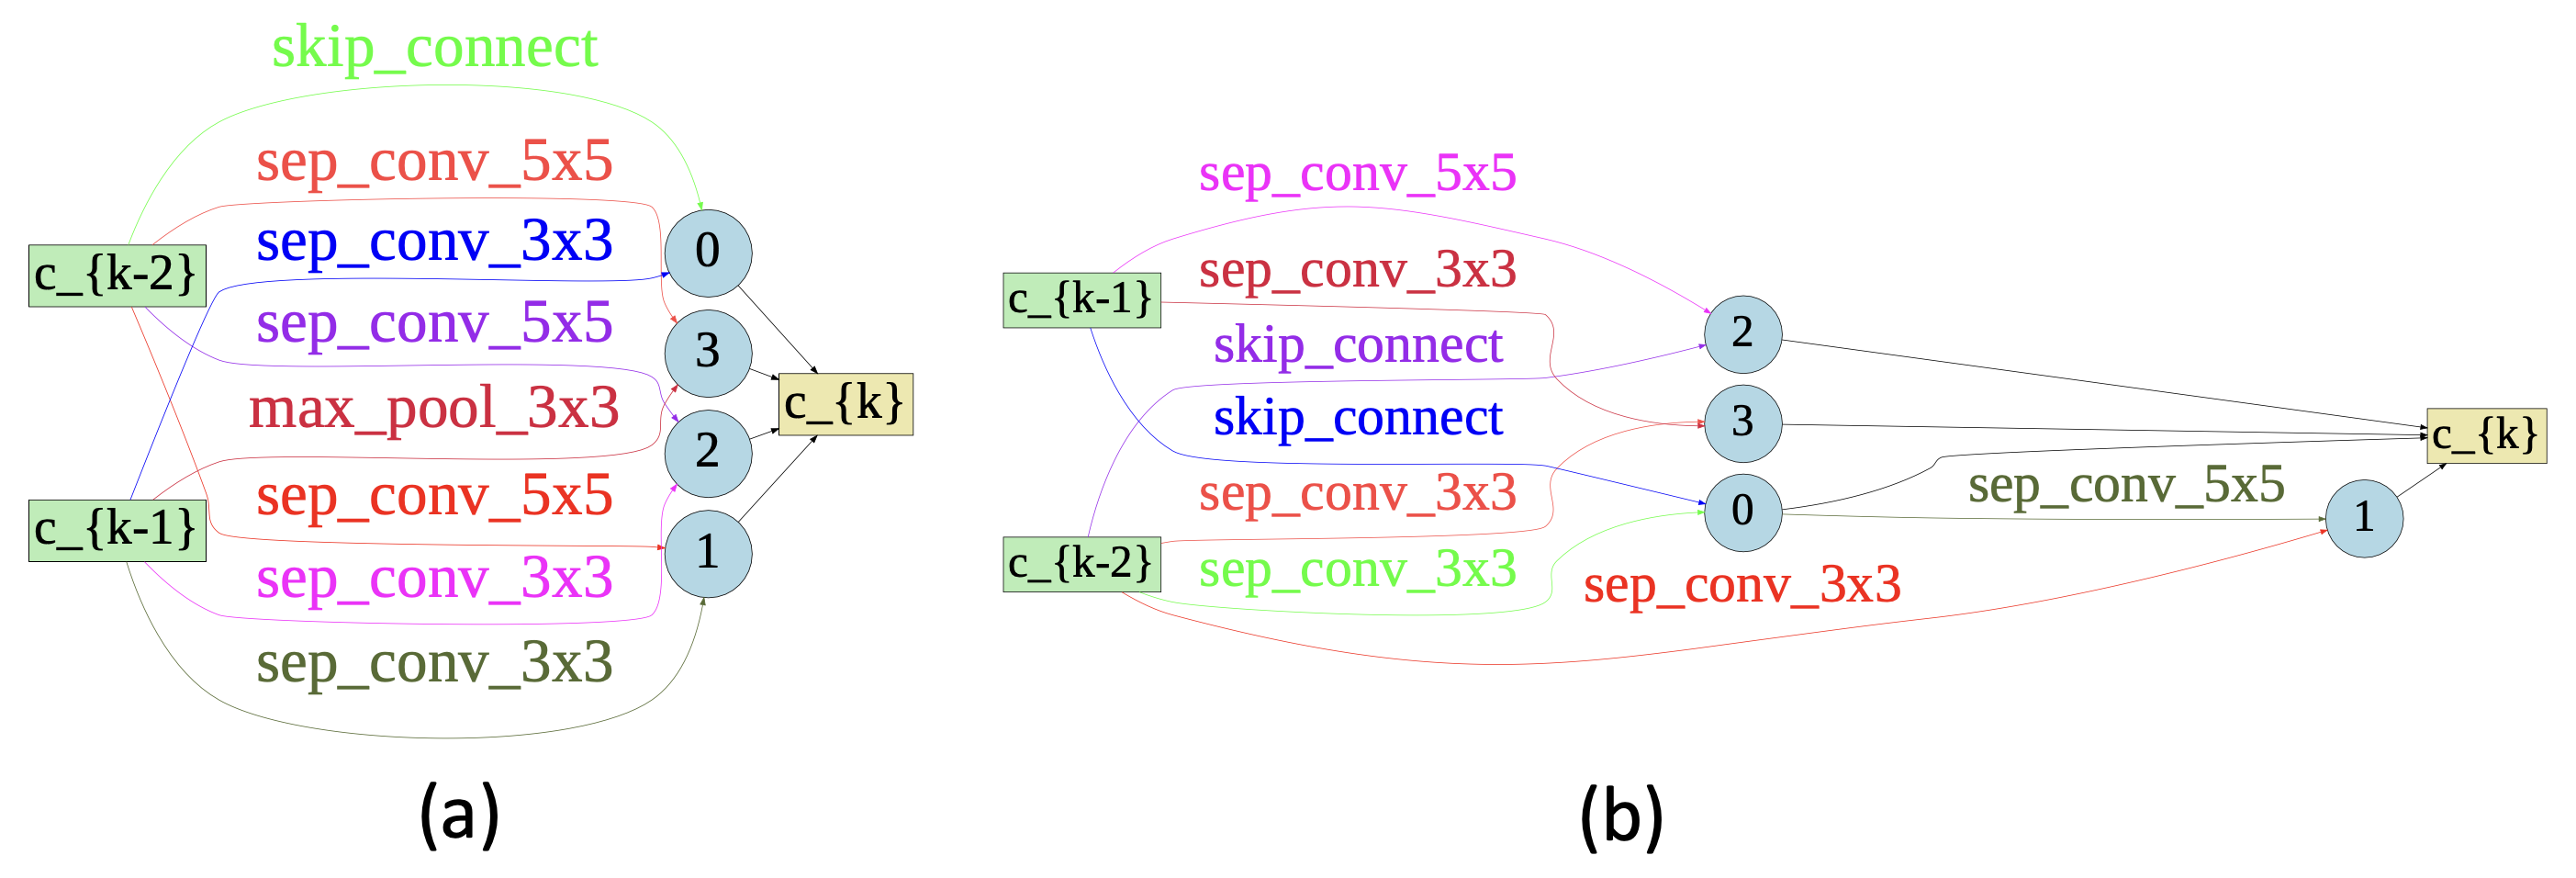
\includegraphics[width=0.6\textwidth]{Figure-4.png}
	\caption{Best cells obtained using (a) supernet and (b) evolutionary approach with CIFAR10 error rates of 2.65\% and 2.49\%, respectively.}
	\label{fig:best_cells}
\end{figure}
next edge, and repeat the valuation. Starting from the random selection of operations on all edges, the model evolves over time since each discretization step improves the operation selected for an edge. After every edge is valued using this successive expansion followed by the valuation technique, each discrete model \( i \) gives a valuation matrix \( V(i) \), which corresponds to the values of search space operations within that discrete model. The valuation matrices from the \( n \) models are averaged to obtain the average valuation of the operations. We only utilize this evolutionary approach in the coarse-grained operation search phase since this stage forms the memory bottleneck due to the expensive supernet training.

\section{EXPERIMENTS AND ABLATION STUDIES}
This section studies the experiments and results of our approach on CIFAR10, NASBench-301, and ImageNet2012. We highlight the importance of search space scalability and, correspondingly, the memory consumption of search. We also perform ablation studies to validate perturbations as an accurate operation evaluation technique.

\subsection{CIFAR10 – Full Search}
This section details experiments for cell search on CIFAR10. We perform search using both the supernet-based and the evolutionary approach (Fig.~\ref{fig:flowchart_search}) to show the difference in accuracy and memory consumption of the two approaches.

\subsubsection{Experimental Setup}
Most of our hyperparameter settings are similar to those utilized by \cite{Liu2018} and \cite{Wang2021} to allow fair comparison of results. We perform our experiments on the DARTS search space \( O_D \). We found the search results of the evolutionary approach to exceed that of the supernet-based approach using only \( n = 4 \) models in the initial population. The search follows the progression detailed in Sec. II-A and Fig.~\ref{fig:flowchart_search}, whereby a coarse-grained operation search phase selects top-2 operations for each edge, followed by a fine-grained operation search, and then the topology search. We repeat the search process with different random seeds four times to ensure consistency in evaluating results compared to previous works.

\subsubsection{Evaluation}
Evaluation follows the same settings as most existing DARTS-like works for consistency of comparison. We utilize 20 cells, with reduction cells at 1/3 and 2/3 of the depths of the model, where reduction cells have the same architecture as normal cells but with stride-2 operations. We train the models for 600 epochs with stochastic gradient descent, 36 initial channels, auxiliary towers with weight 0.4, and cutout with length 16. We report and compare the average and best accuracy of the four runs in Table.~\ref{comparison_1}. All works below the double horizontal line in Table.~\ref{comparison_1} utilize the DARTS search space. Architectures of the best searched cells of the four runs from the supernet-based and evolutionary approach are shown in Fig.~\ref{fig:best_cells}. ProxylessNAS \cite{Cai2018} achieves 0.41\% and 0.03\% better accuracy on CIFAR10 and ImageNet, respectively, than the best cell found using our approach. However, the search cost of 8.3 GPU days, combined with model sizes roughly 1.4× that of our results, makes the approach less appealing. Furthermore, ProxylessNAS has not been applied to DARTS-like search spaces, which makes the comparison inequitable.

\begin{table}[ht]
	\centering
	\caption{Performance Comparison against the State-of-the-Art on CIFAR10 and ImageNet2012}
	\label{comparison_1}
	\resizebox{\textwidth}{!}{
		\begin{tabular}{lccccccc}
			\hline
			Work & Error CIFAR10(\%) & Params CIFAR (M) & Error Top 1 & ImageNet Top 5 & Params ImgNet (M) & Search Time CIFAR (GPU Days) & Peak GPU Mem (GB) ‡\\ \hline
			NASNet-A \cite{Zoph2018} & 2.65 & 3.3 & 26.0 & 8.4 & 5.3 & 1800 & -\\
			AmoebaNet-B \cite{Real2019} & 2.55 $\pm$ 0.05 & 2.8 & 26.0 & 8.5 & 5.3 & 3150 & -\\
			ENAS \cite{Pham2018} & 2.89 & 4.6 & - & - & - & 0.5 & -\\
			PNAS \cite{Liu2018Progressive} & 3.41 $\pm$ 0.09 & 3.2 & 25.8 & 8.1 & 5.1 & 225 & -\\
			ProxylessNAS \cite{Cai2018} & 2.08 & 5.7 & 24.9 & 7.5 & - & 8.3 & -\\ \hline \hline
			SNAS \cite{Xie2018} & 2.85 $\pm$ 0.02 & 2.8 & 27.3 & 9.2 & 4.3 & 1.5 & 33.1\\
			PC-DARTS (Reproduced) \cite{Xu2019} & 2.84† $\pm$ 0.09 & 3.6 & 25.1 & 7.8 & 5.3 & 0.1 & 11.8\\
			R-DARTS \cite{Zela2019} & 2.95 $\pm$ 0.21 & - & - & - & - & 1.6 & 32.6\\
			SGAS \cite{Li2020SGAS} & 2.66 $\pm$ 0.24 & 3.7 & 26.0 & 8.5 & 5.3 & 0.3 & 32.6\\ \hline
			DARTS \cite{Liu2018} & 3.00 $\pm$ 0.14 & 3.3 & 26.7 & 8.7 & 4.7 & 0.4 & 32.6\\
			DARTS+PT (avg) \cite{Wang2021} & 2.61 $\pm$ 0.08 & 3.0 & - & - & - & 0.8 & 32.6\\
			DARTS+PT (best) \cite{Wang2021} & 2.48 & 3.3 & 25.5 & 8.0 & 4.6 & 0.8 & 32.6\\
			PertNAS (Supernet) (avg) & 2.69 $\pm$ 0.04 & 3.9 & - & - & - & 0.2 & 17.8\\
			PertNAS (Supernet) (best) & 2.65 & 4.1 & - & - & - & 0.2 & 17.8\\ \hline
			\textbf{PertNAS (Evolutionary) (avg)} & 2.58 $\pm$ 0.08 & 4.1 & - & - & - & 0.2 & 6.2\\
			\textbf{PertNAS (Evolutionary) (best)} & 2.49 & 4.0 & 25.2 & 7.8 & 5.6 & 0.3 & 6.2\\ \hline
		\end{tabular}
	}
	\\
	\vspace{0.2cm}
	\footnotesize{
		\begin{minipage}{\textwidth}
			\raggedright
			† Authors’ reported accuracy: 2.57\%, Reproduced accuracy using authors’ official implementation: 2.84\%. \\
			‡ Measured using an A100 GPU, PyTorch 1.12 + CUDA 11.3 @ batch size 256.
		\end{minipage}
	}
	\end{table}

	
	\begin{table}[ht]
		\centering
		\caption{Performance Comparison on NASBENCH-301, and the GPU-Memory Consumption for Search on CIFAR10}
		\label{comparison_2}
			\begin{tabular}{lccc}
				\hline
				Work & Accuracy (\%) & Params (M) & Peak GPU Mem (GB) \\ \hline
				SNAS \cite{Xie2018} & 94.22 & 2.8 & 33.1 \\
				PC-DARTS \cite{Xu2019} & 94.03 & 3.6 & 11.8 \\
				SGAS \cite{Li2020SGAS} & 94.31 & 3.8 & 32.6 \\
				DARTS \cite{Liu2018} & 93.68 & 3.3 & 32.6 \\
				DARTS+PT \cite{Wang2021} & 93.84 & 3.3 & 32.6 \\
				PertNAS (Supernet) & 94.58 & 4.1 & 17.8 \\ \hline
				\textbf{PertNAS (Evolutionary)} & 94.71 & 4.0 & 6.2 \\ \hline
			\end{tabular}
		

	\end{table}


Our evolutionary scheme exceeds the average accuracy achieved by PC-DARTS \cite{Xu2019} by 0.26\% and requires only around 0.5× the memory. Against DARTS+PT, we achieve comparable accuracy with almost 1/4 the search time while utilizing less than 1/5 the memory.

\subsection{NASBench-301}
We compare the performance of the best-generated cells under both search schemes against SoTA DARTS-like works on NASBench-301 \cite{Siems2020}. NASBench-301 is a surrogate benchmark that allows comparing the performance of NAS works without expensive model training. We utilize the two best cells obtained as a result of search on CIFAR10 (Sec. IV-A, Fig.~\ref{fig:best_cells}) to perform the evaluation on NASBench. Table.~\ref{comparison_2} shows that the best cells generated using the evolutionary approach exceed DARTS \cite{Liu2018} by 1.03\%, PC-DARTS \cite{Xu2019} by 0.68\%, and DARTS+PT \cite{Wang2021} by 0.87\%. The corresponding cells, shown in Fig.~\ref{fig:best_cells}, are rich in learnable parameters as they contain many convolutions, leading to large model sizes. Existing works have shown that searched model accuracies are proportional to their sizes \cite{Zela2020, Siems2020} as will also be shown in Sec. IV-E and Fig.~\ref{fig:search_comparison} (a). Furthermore, high-quality models utilize separable as opposed to dilated convolutions \cite{Siems2020}, and shallow as opposed to deep cells, as exhibited by our searched cells in Fig.~\ref{fig:best_cells}.

\subsection{Transferability Evaluation on ImageNet}
We test the transferability of cells found on CIFAR10 to the ImageNet dataset. This test follows the mobile setting for evaluation whereby the number of multiply-add operations in the model is restricted to be less than 600M, with an input size of 224x224. The remaining hyperparameters also follow the configuration utilized by previous works for fair comparison \cite{Liu2018, Wang2021}. Comparison of top-1 and top-5 accuracy achieved on ImageNet under transferability evaluation of cells found on CIFAR10 against some state-of-the-art works is shown in Table.~\ref{comparison_1}. We achieve 0.3\% better top-1 accuracy compared to DARTS+PT owing to the parameter-rich cells resultant from our approach. Against ProxylessNAS, we achieve 0.3\% worse top-1 accuracy but with a search time of only 0.3 GPU-days. Against PC-DARTS, we achieve 0.1\% worse top-1 accuracy. However, PC-DARTS performs search directly on each dataset, with a search on ImageNet costing 3.8 GPU-days, roughly 13× our search time. Hence, our approach produces results comparable to the SoTA with minimal search cost in both time and memory.

\subsection{Importance of Search-Space and Memory Scalability}
The evolutionary approach allows the evaluation of the search space from within discrete models. Hence, the peak memory consumption of our evolutionary approach is similar to that of training a compact model sampled from the search space. We evaluate the peak memory allocated to search at different search space sizes using supernet-based and evolutionary techniques. We also showcase the importance of scaling up the search space by analyzing its impact on the quality of searchable architectures. Starting from \( O = \{ \text{none}, \text{skip connect}, \text{max pool } 3 \times 3, \text{avg pool } 3 \times 3 \} \), i.e., the subset of the DARTS search space with \( |O| = 4 \), we scale up the search space by adding convolution operations with different kernel sizes into the search space, e.g., to make \( |O| = 5 \), we add a sep conv \( 3 \times 3 \) into \( O \). At each \( |O| \), we obtain the average accuracy of up to 10k randomly sampled models from the search space on NASBench-301, whereby a fixed shallow search space topology, similar to \( O_1 \) in Table.~\ref{tab:search_spaces}, is utilized. This average accuracy denotes the quality of searchable models in the search space; higher average accuracy implies that search methods can potentially generate high-quality models from the search space. However, we can only obtain average accuracies for search space sizes up to \( |O| = 7 \) due to limitations on the operations available in NASBench-301. We also measure the peak reserved memory for search, composed of memory allocated to tensors, cached memory, and CUDA context. The results in Fig.~\ref{fig:gpu_memory_consumption} show that while the GPU memory requirement for supernet-based search (e.g., DARTS-like approaches that rely on supernets) increases almost linearly with search space size, the memory requirement of the evolutionary approach stays almost constant. Hence, our approach offers possibilities for scaling the search space significantly, sidestepping the hardware limits imposed by supernet-based approaches like DARTS. This scalability is essential since larger search spaces hold more high-quality models, as depicted by the increasing average accuracy of models with increasing search space sizes \( |O| \).

\begin{figure}[ht]
	\centering
	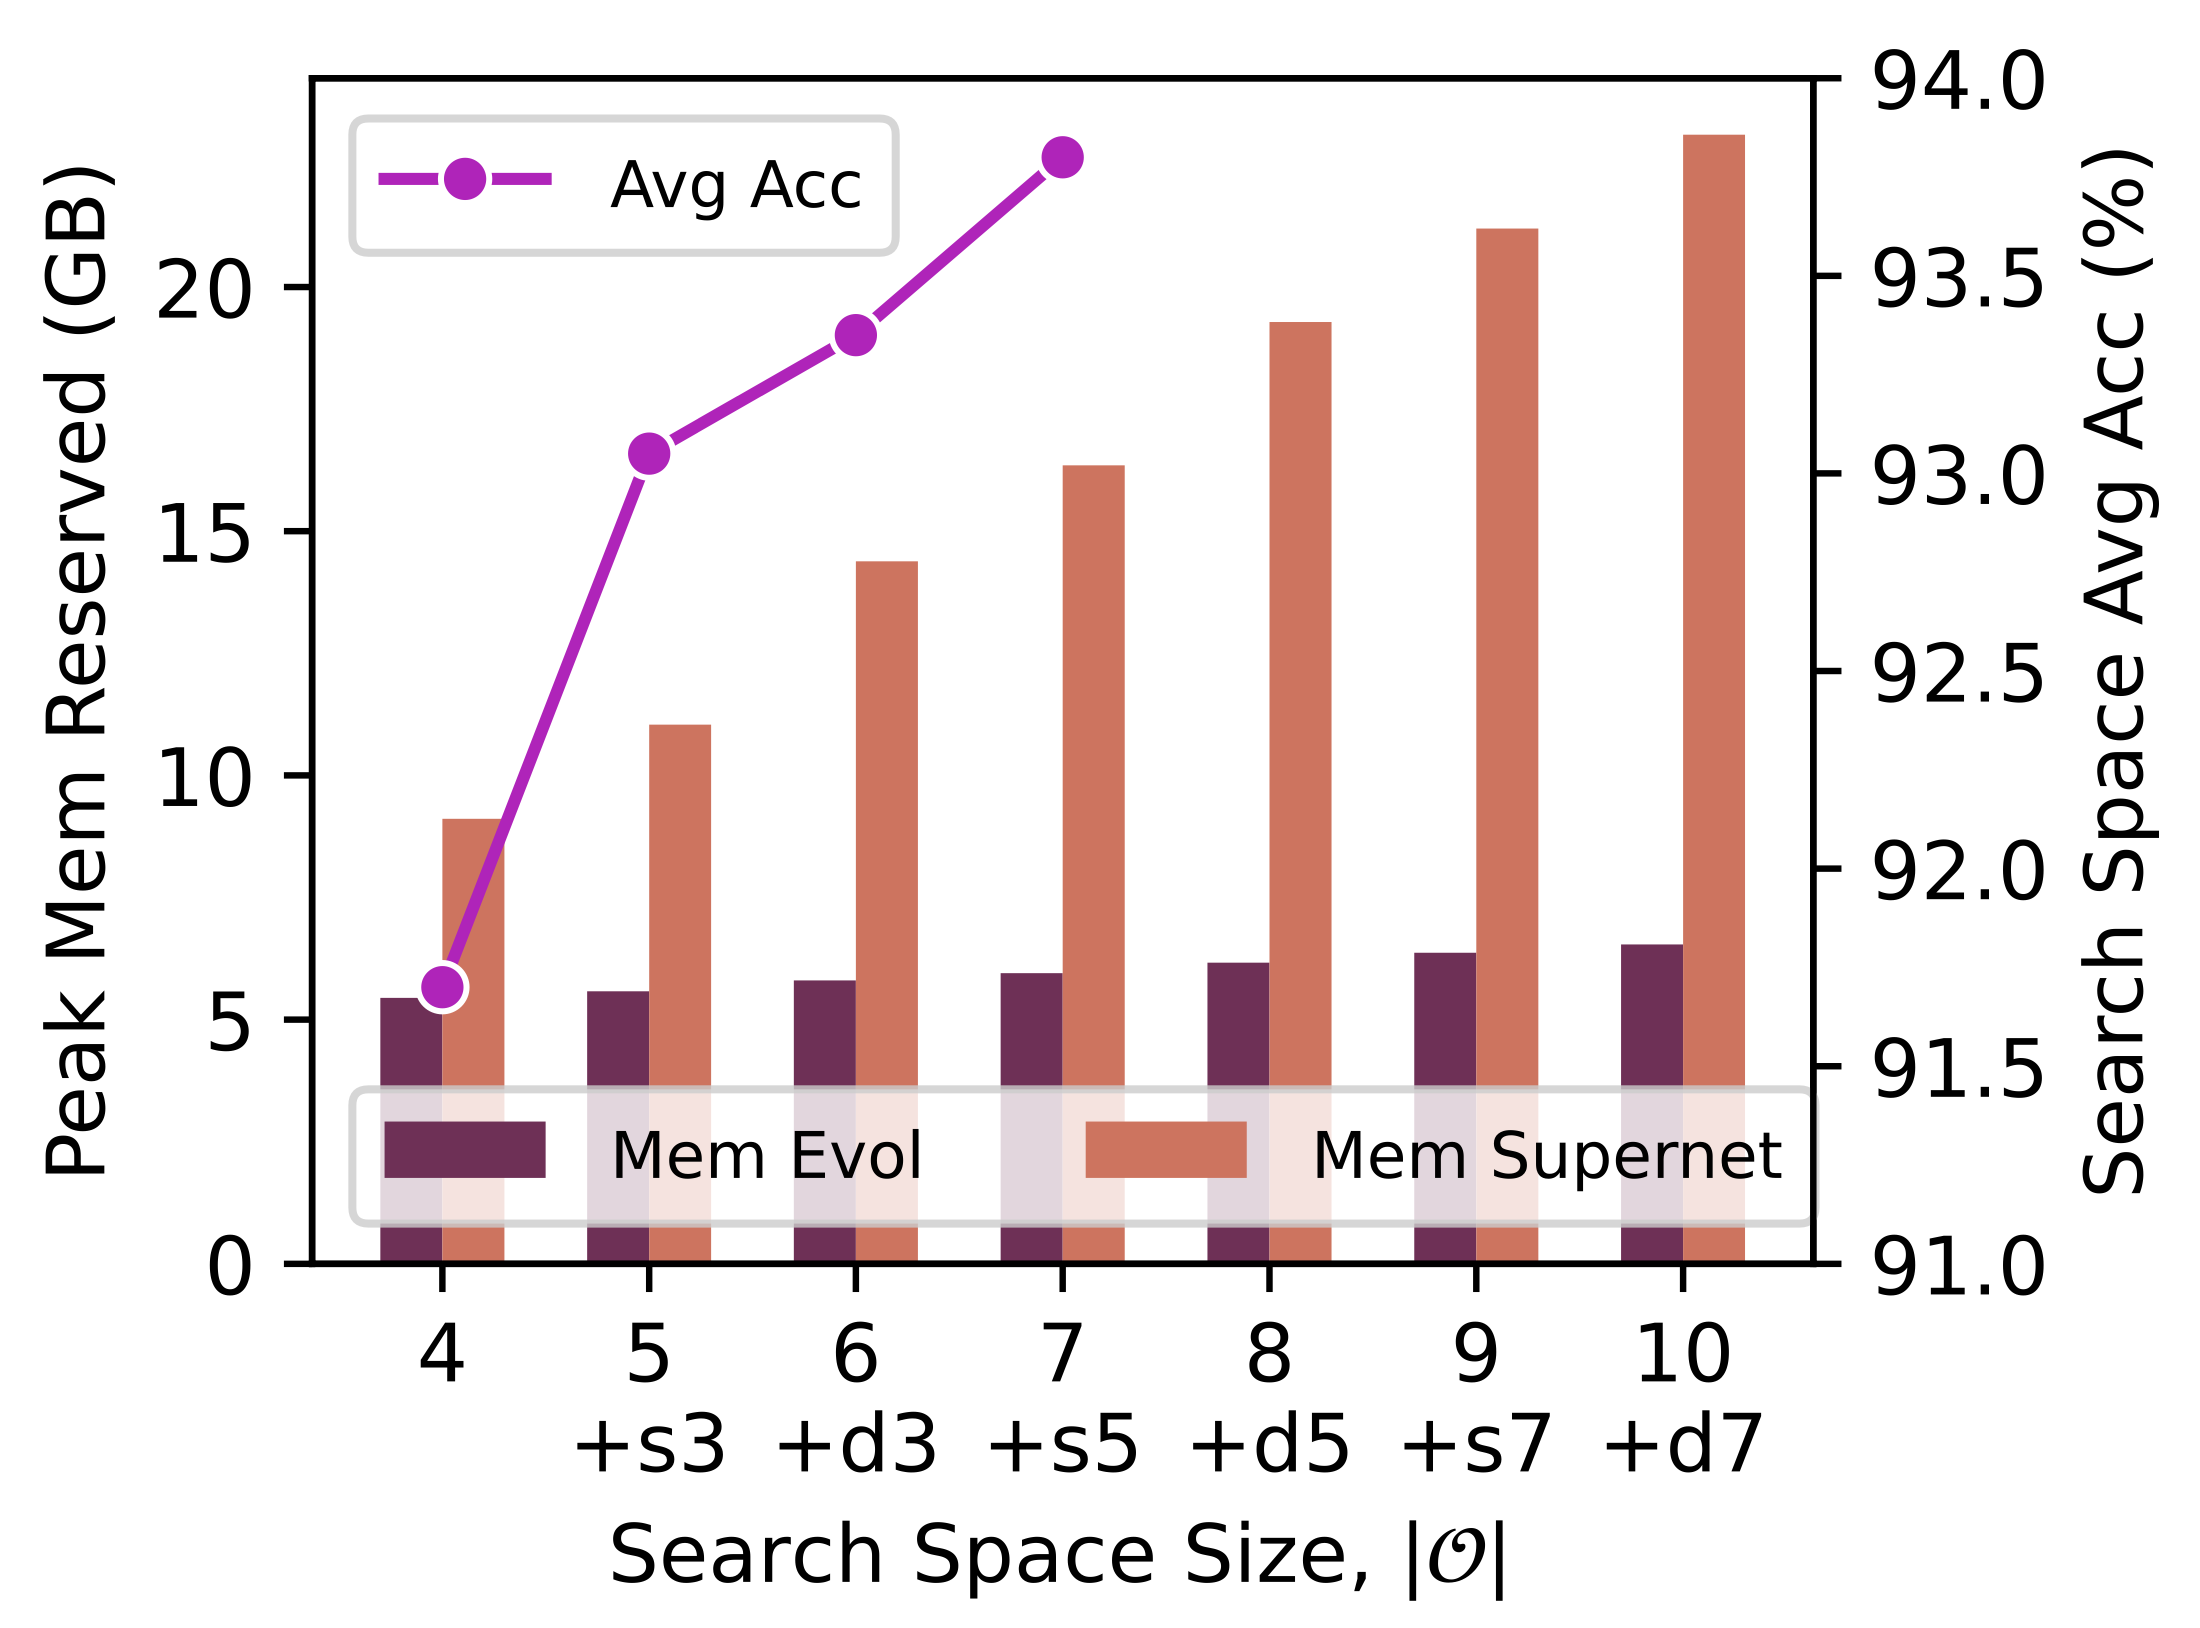
\includegraphics[width=0.45\textwidth]{Figure-5.png}
	\caption{Bar chart of GPU-memory consumption for search on search spaces of different sizes. Also shown is the average accuracy of 10k randomly chosen models in the search spaces (s3=sep conv 3x3, d3=dil conv 3x3). The notation +s3 indicates that the search space size is increased by adding a sep conv 3x3 operation to the preceding O.}
	\label{fig:gpu_memory_consumption}
\end{figure}
	
\subsection{Ablation 1 – Fidelity of Perturbations for Operation Search}
This ablation study explores the validity of perturbations-based operation search. We utilize search space \( O_1 \) with NASBench-301 for this study due to its fixed topology and the availability of ground truth valuation of operations in the search space. To perform search using the perturbations-based approach, we randomly sample a total of \( n = 8 \) discrete models from the search space. We train each of the discrete models to convergence, expand and value each edge using perturbations, average the valuation matrices obtained from each of the 8 models, and select the top \( o,e \) pair from the cell and discretize \( e \) to \( o \). We repeat this process for the remaining edges until the best operation for each edge is selected. To compare the results of operation search on \( O_1 \) against previous works, we perform similar searches using DARTS \cite{Liu2018} and DARTS+PT \cite{Wang2021}. Figure~\ref{fig:search_comparison} (a) shows the accuracy of all $\sim 65k$ models in the search space and compares the accuracy of models obtained using the three different approaches: DARTS, DARTS+PT, and PertNAS. The cells resultant from our approach consist of 7 sep conv operations, leading to higher accuracy and model size compared to DARTS+PT and DARTS.

\subsection{Ablation 2 – Fidelity of Perturbations for Topology Search}
For evaluation of perturbations for topology search, we utilize the search space of \( O_2 \) whereby we enumerate all possible topologies that can be constructed from the best operation choices in \( O_1 \). This corresponds to a total of only 180 topologies, with their accuracies on NASBench-301 \cite{Siems2020}, and cell depths shown in Fig.~\ref{fig:search_comparison} (b). Shallower DARTS cells perform better, as also validated by \cite{Siems2020}. We construct a supernet consisting of all 14 possible edges in each cell, with each edge consisting only of the top operation from \( O_1 \). We apply topology search on this supernet using perturb-valuation of all edges and selecting the top-2 incoming edges for each intermediate node. Results in Fig.~\ref{fig:search_comparison} (b) show that the topology obtained using this valuation scheme is among the top 5 topologies in this search space and achieves 0.16\% better accuracy at the same model size as DARTS+PT \cite{Wang2021}.

\section{CONCLUSION}
This paper proposed a perturbations-based approach to evaluating search space components in NAS. We showed how perturbations can be applied to discrete models in an evolutionary search scheme to allow the valuation of search space in a memory-efficient fashion. The evolutionary approach disentangles memory consumption from search space size, overcoming the constraints imposed by hardware limits on search spaces. Experiments using CIFAR10, NASBench-301, and ImageNet show a competitive performance of perturbations-based search relative to differentiable approaches, at roughly only 20\% of their memory costs. Our approach is fast, accurate, and scalable to larger search spaces. It generates architectures that conform to our understanding of high-quality architectures in the search space, such as shallow and parameter-rich cells.

\begin{figure}[ht]
	\centering
	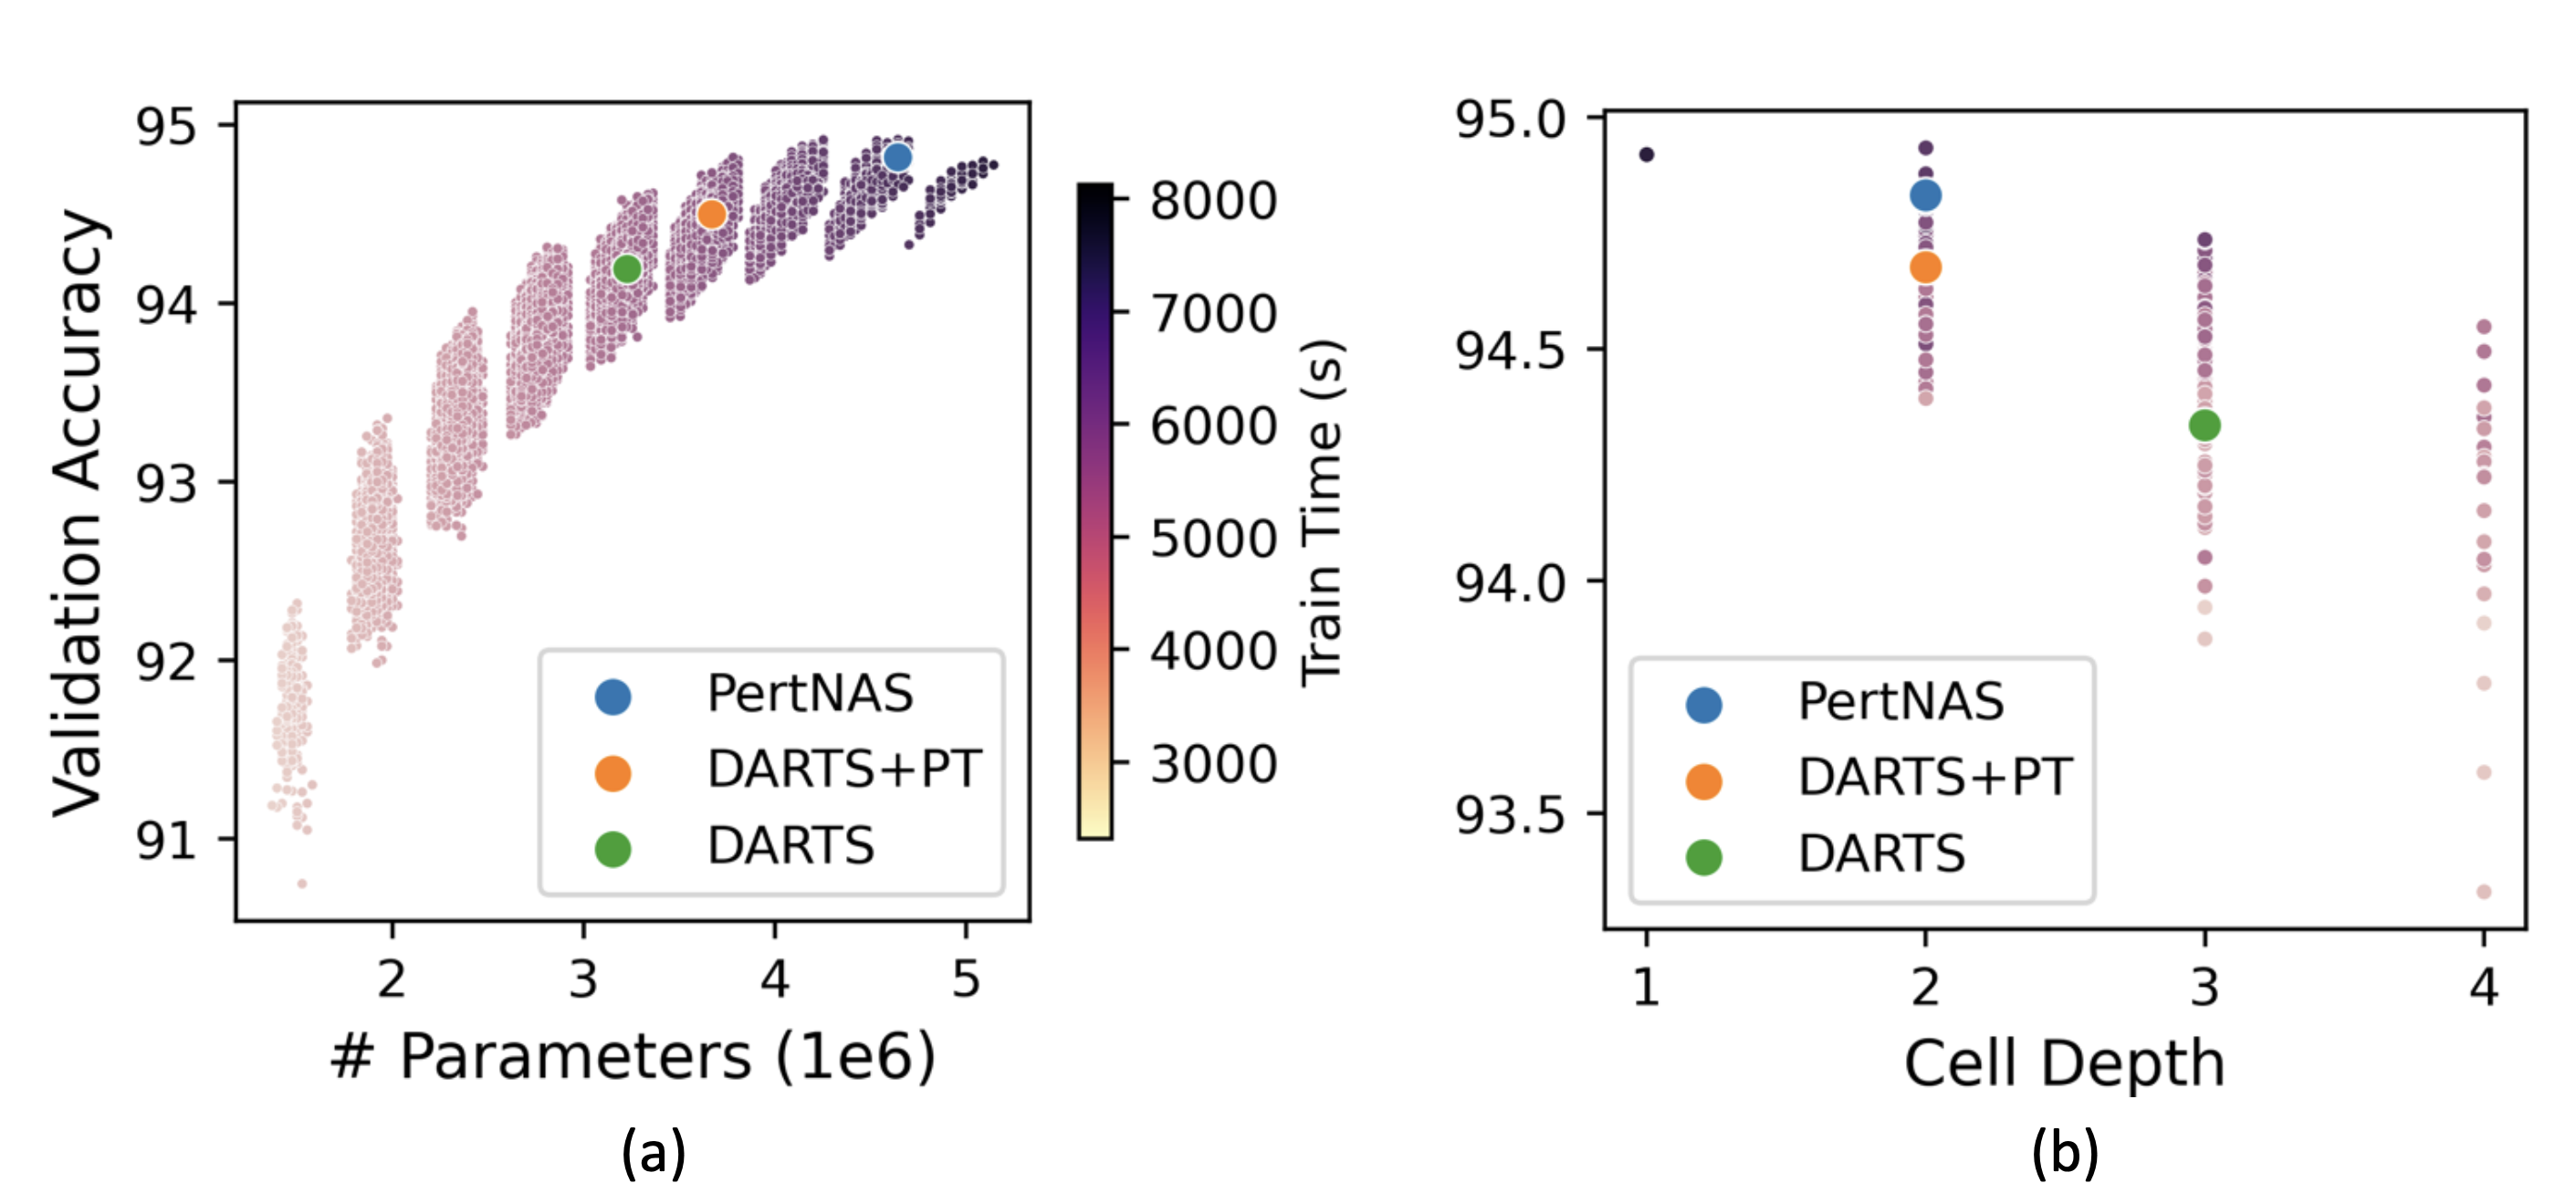
\includegraphics[width=0.8\textwidth]{Figure-6.png}
	\caption{Comparison of results from operation and topology searches on CIFAR-10 using NASBench-301 against DARTS \cite{Liu2018} and DARTS+PT \cite{Wang2021}. (a) Operation Search Space O1 with 65.5k models. (b) Topology Search Space O2 with only 180 models, plotted against cell depth. The hue represents training time.}
	\label{fig:search_comparison}
\end{figure}
\section*{ACKNOWLEDGEMENTS}
This research was partially supported by ACCESS - AI Chip Center for Emerging Smart Systems, Hong Kong SAR. The authors also acknowledge compute support from Cloudlab \cite{Duplyakin2019} and Turing AI Compute Cluster (TACC).


\bibliographystyle{IEEEtran}
\bibliography{1}

\end{document}